% !TeX root = vpl.tex

\chap{Il robot trova la strada da solo}\label{ch.line}

Un'escursione in montagna è una semplice attività:
prendi un paio di scarpe da trekking e segui un percorso.
Per un robot, seguire un percorso a terra può anche essere molto utile.
Si consideri un magazzino con carrelli robotizzati che portano gli oggetti in una zona centrale di dispacciamento.
Ci sono linee tracciate sul pavimento del magazzino e il robot riceve istruzioni di seguire
alcune linee fino a raggiungere lo scomparto di archiviazione dell'oggetto desiderato.
Per farlo, il robot deve vedere queste righe.
Scriviamo ora un programma che faccia in modo che il robot segua una linea sul pavimento.

{\raggedleft \hfill File di programma \bu{follow-line.aesl}}

Il compito di seguire una linea mette in evidenza tutta l'incertezza di costruire
robot nel mondo reale: Il robot deve affrontare l'incertezza delle sue percezioni
e delle sue azioni.
Per esempio, la linea potrebbe non essere perfettamente rettilinea, la polvere può oscurare parte della linea, o la sporcizia può fare in modo che una ruota si muova più lentamente rispetto all'altra.
Per seguire una linea, il robot deve utilizzare un
\emph{controller}  che decide quanta potenza applicare per ogni motore
a seconda dei dati ricevuti dai sensori.

\sect{La linea e il robot}

\begin{figure}
	\subfigure[Thymio segue una striscia di nastro]{ \label{fig.tape} 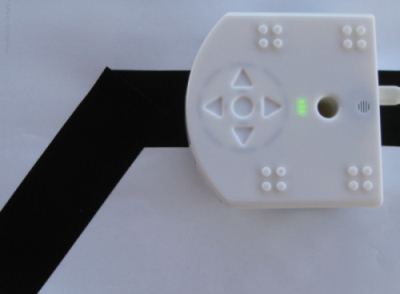
\includegraphics[height=0.35\textwidth]{blacktape}}
	\hfill
	\subfigure[Il sensore sinistro è fuori dal nastro e il sensore destro è sul nastro]{ \label{fig.one-off} 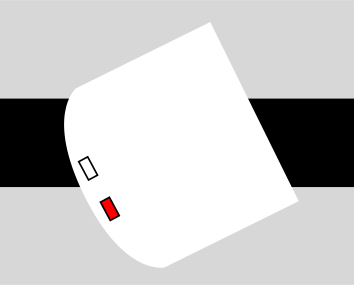
\includegraphics[height=0.35\textwidth]{thymio_half_on_line}}
	\caption{Thymio su un nastro nero}
\end{figure}

Per seguire una linea, usiamo i sensori di terra (\cref{ch.moving}).
Ricorda che questi funzionano con l'invio di luce infrarossa (invisibile all'occhio umano) e misurano quanto viene riflessa indietro.
Se il pavimento è di colore chiaro, il sensore rileverà molta luce riflessa
e si verificherà  l'evento \blksm{lots-of-light}. Abbiamo bisogno di una linea
che causi l'evento poca luce riflessa
\blksm{little-light}. Questo è facile da fare stampando una linea nera, dipingendo o mettendo nastro isolante nero sul pavimento (\cref{fig.tape}). La linea deve
essere sufficientemente ampia in modo che entrambi i sensori di terra leggano il nero quando il
robot segue correttamente la linea. Una larghezza di 5
centimetri è sufficiente per fare in modo che il robot segua la linea, anche se ci
sono piccole deviazioni.

In primo luogo, facciamo andare avanti Thymio ogni volta che \emph{entrambi}  i sensori rilevano
una superficie scura (il robot è sulla linea) e lo facciamo fermare ogni volta che \emph{entrambi}  i sensori rilevano un
superficie di luce (il robot non è la linea).
Le coppie evento-azione sono riportati nella \cref{fig.start-stop}.

\trickbox{Assicurarsi di utilizzare un cavo USB che sia abbastanza lungo (diciamo, due
metri), in modo che Thymio possa restare collegato al computer anche
quando si sposta.
È possibile trovare le prolunghe in qualsiasi negozio di computer.}


\begin{figure}
	\subfigure[Avvia e ferma il robot]{ \label{fig.start-stop} 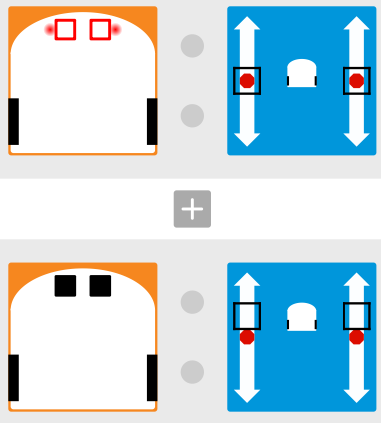
\includegraphics[width=0.4\textwidth]{line-forward}}
	\hfill
	\subfigure[Correggi le deviazioni]{ \label{fig.follow-line} 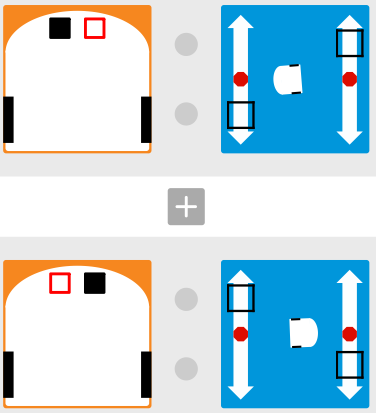
\includegraphics[width=0.4\textwidth]{line-controller}}
	\caption{Un programma per seguire una linea}
\end{figure}

\sect{Il vostro primo controller}

Il passo successivo è quello di programmare il controller che segue la linea::
\begin{itemize}

\item Se il robot si muove fuori dal nastro a \emph{sinistra}, come in \cref{fig.one-off}, il
 sensore di \emph{sinistra} rileverà il pavimento mentre il sensore di \emph{destra}
sta ancora rilevando il nastro; in tal caso il robot deve ruotare leggermente
a \emph{destra}.
\item Se il robot si muove fuori dal nastro a \emph{destra}, il
 sensore di \emph{destra} rileverà il pavimento mentre il sensore di \emph{sinistra}
sta ancora rilevando il nastro; in tal caso il robot deve ruotare leggermente
a \emph{sinistra}.

\end{itemize}

Sono necessarie due coppie evento-azione, come mostrato in \cref{fig.follow-line}.

\sect{Fissare i parametri}

E' facile vedere che se il robot scappa dal bordo sinistro del nastro, si deve girare a destra, come in \cref{fig.one-off}.
La vera domanda è quanto stretta deve essere la curva?
Se la curva è troppo dolce, \emph{anche} il sensore di destra potrebbe uscire dal nastro prima che il robot torni indietro;
se la curva è troppo aggressiva, potrebbe far uscire il robot dall'altro lato del nastro. In ogni caso, curve aggressive possono essere pericolose per il robot e tutto ciò che sta portando.

In questo programma, è possibile impostare le velocità dei
motori di destra e di sinistra in ogni blocco azione motori. Avrete bisogno di
fare un po' di prove con questi valori fino a quando il robot segua in modo \emph{affidabile} la linea. Affidabile qui
significa che il robot riesce a seguire con successo la linea più volte.
E' necessario eseguire
diversi test per assicurarsi che il programma funzioni, mettendo il robot sulla linea in una posizione leggermente diversa e
che punti in una direzione leggermente diversa.

Ci sono molti modi per configurare i blocchi di azione motori.
La velocità di avanzamento del robot sulla linea è un parametro importante.
Se è troppo veloce, il robot può scappare dalla linea prima che le azioni di correzione possano influenzare la sua direzione. Tuttavia, se la velocità è troppo lenta, nessuno comprerà il vostro robot da utilizzare in un magazzino.

Se il Thymio esce dalla linea, che cosa dovrebbe fare?
Se fa una brusca virata (un motore va avanti e l'altro indietro),
il robot ritorna rapidamente sulla linea, però i suoi movimenti saranno molto a scatti.
D'altra parte, se il robot fa una curva dolce (un motore va leggermente più veloce rispetto all'altro), il robot si sposta uniformemente ma può perdere la linea.
Dovrete sperimentare per trovare buoni compromessi.

\newpage

\exercisebox{\thechapter.1}{
Il robot si arresta quando entrambi i sensori del terreno rilevano che sono fuori dal
nastro. Modifica il programma in modo che il robot faccia una dolce svolta a sinistra nel tentativo di trovare nuovamente il nastro. Provalo su un nastro con una svolta a sinistra
come quello mostrato in \cref{fig.tape}. Provare ad aumentare la
velocità in avanti del robot. Cosa accade quando il robot arriva alla fine del
nastro?
}

\vfill

\exercisebox{\thechapter.2}{
Modifica il programma dall'esercizio precedente in modo che
il robot giri a destra quando viene perso il nastro. Che succede?
\vspace{.5em}\\
Sarebbe bello se potessimo \emph{ricordare}  quale sensore è stato l'ultimo
a perdere il contatto con il nastro in modo da far sterzare il robot nella direzione giusta per ritrovare il nastro. Nel 
\cref{ch.states}
impareremo come Thymio possa ricordare le informazioni.
}

\vfill

\exercisebox{\thechapter.3}{
Esperimenta con diverse disposizioni delle linee di nastri:
\begin{itemize}[noitemsep,nosep,leftmargin = *]
\item curve ampie;
\item curve strette;
\item linee a zig zag;
\item linee più ampie;
\item linee più strette.
\end {itemize}
Organizza delle gare di corsa con i tuoi amici: quale robot segue con successo la
maggior parte delle linee? Per ogni linea, quale robot la segue nel tempo più breve?
}



\vfill

\exercisebox{\thechapter.4}{
Discutere che effetto le seguenti modifiche di Thymio potrebbero
avere sulla capacità del robot di seguire una linea:
\begin{itemize}[noitemsep,nosep,leftmargin=*]
\item gli eventi di rilevamento dei sensori del terreno si verificano più spesso o meno spesso di 10 volte al secondo;
\item i sensori sono più lontani o più vicini;
\item ci sono più di due sensori di terra nella parte inferiore del robot.
\end{itemize}
}
